% an empty .tex file. Eventually may transfer .odt in here
%%This is a very basic article template.
%%There is just one section and two subsections.
%\documentclass[12pt,oneside,a4paper,doublespacing]{article} % for submission
\documentclass[11pt,oneside,a4paper]{article} % for sharing

\usepackage{appendix}
\usepackage{amsmath}
\usepackage{caption}
\usepackage{placeins}
\usepackage{graphicx}
\usepackage{subcaption}
%\usepackage{subfig}
\usepackage{longtable}
\usepackage{setspace}
%\usepackage{tikz}
\usepackage{booktabs}
\usepackage{tabularx}
\usepackage{xcolor,colortbl}
\usepackage{chngpage}
%\usepackage[active,tightpage]{preview}
\usepackage{natbib}
\bibpunct{(}{)}{,}{a}{}{;} 
\usepackage{url}
\usepackage{nth}
\usepackage{authblk}
\usepackage[most]{tcolorbox}
%\usepackage{hyperref}
%\usepackage{color}
%\usepackage{fontspec}
%\usepackage{pdfsync}
\usepackage[normalem]{ulem}
\usepackage{amsfonts}
\renewcommand{\listtablename}{List of Appendix Tables}
\newcolumntype{C}[1]{>{\centering\let\newline\\\arraybackslash\hspace{0pt}}m{#1}}
\newcolumntype{L}[1]{>{\raggedright\let\newline\\\arraybackslash\hspace{0pt}}m{#1}}
% working on this need to concatenate file name based on sex and variable name
%\newcommand\Cell[1]{{\raisebox{-0.05in}{\includegraphics[height=.2in,width=.2in]{Figures/ColorCodes/\expandafter#1}}}}  

%%%%%%%%%%%%%%%%%%%%%%%%%%%%%%%%%%%%%%%%%%%%%%%%%%%%%%%%%%%%%%%%%%%%%%%%%%%%%
% setting color to letters affects spacing. Here's a hack I found here:
% http://tex.stackexchange.com/questions/212736/change-letter-colour-without-losing-letter-spacing
%\DeclareRobustCommand{\spacedallcaps}[1]{\MakeUppercase{\textsc{#1}}} % all
% caps with better spacing

%\colorlet{RED}{red}
%\colorlet{BLUE}{b}
\colorlet{rd}{red}
\colorlet{bl}{blue}

%%%%%%%%%%%%%%%%%%%%%%%%%%%%%%%%%%%%%%%%%%%%%%%%%%%%%%%%%%%%%%%%%%%%%%%%%%%%%%

\newcommand\ackn[1]{%
  \begingroup
  \renewcommand\thefootnote{}\footnote{#1}%
  \addtocounter{footnote}{-1}%
  \endgroup
}
\newcommand\vt[1]{\textcolor{rd}{#1}}
\newcommand\eg[1]{\textcolor{bl}{#1}}

\newcommand\tg[1]{\includegraphics[scale=.5]{Figures/triadtable/triad#1.pdf}}
\newcommand\tgh[1]{\raisebox{-.25\height}{\includegraphics[scale=.3]{Figures/triadtable/triad#1.pdf}}}

\defcitealias{HMD}{HMD}

% junk for longtable caption
\AtBeginEnvironment{longtable}{\linespread{1}\selectfont}
\setlength{\LTcapwidth}{\linewidth}

%%%%%%%%%%%%%%%%%%%%%%%%%%%%%%%
\begin{document}

\title{A best practices composite lifetable for US states}

\author[1]{Tim Riffe\thanks{triffe@demog.berkeley.edu}}
\author[2,3]{Adrien Remund}
\author[3,4]{Magali Barbieri}
\author[4]{Celeste Winant}
\affil[1]{Max Planck Institute for Demographic Research}
\affil[2]{universit{\'e} de Gen{\`e}ve}
\affil[3]{Institut National d'{\'e}tudes D{\'e}mgraphiques}
\affil[4]{Department of Demography, University of California, Berkeley}

%\author{[Authors]}

\maketitle

\begin{abstract}
We calculate a preliminary series of best-possible lifetables for the United
States from 1959-2004, defined as the age-specific aggregate of the lowest
observed age-cause specific death rates among the 50
states and the District of Columbia for each year. This synthetic best practices lifetable shows a gradual
increasing trend over the period, on average 1.9 and 2.2 years higher
than the highest state life expectancy in each year for males and females,
respectively. We argue that the US states best practices lifetable is a useful
guage of mortality.
\ackn{The work reported in this manuscript was supported in part by the U.S.
National Institute On Aging of the National Institutes of Health under award
numbers R01-AG011552 and R01-AG040245. The content is solely the responsibility of the authors and does not necessarily represent the official views of the funding agencies.}
\end{abstract}


\section*{Introduction}

The question of limits to life expectancy is fundamental to demography, but it
is also practical when projecting mortality. Mortality reductions in past
decades have been steady in many populations, and at times linear, which tends
to guide projections into predicting the same sort of progress far into the
future. Most past attempts to place limits on such projections were shown to be
overly conservative within a short period of years \citep{oeppen2002broken}.
However, many simple mortality projections will send life expectancy scenarios
to very high levels that for a given population may seem unimaginable. In some
cases, one seeks an external population that has already achieved a life
expectancy as high as that produced by a model, and this gives some assurance
that the projection is possible. Japan assumes this role in many cases today. In
2012 life expectancy for Japanese females was 86, while for US females it was 81
\citep{HMD}. If a US projection turns out to reach 86 we at least know that this
is indeed possible.

The desire for such external references explains part of the interest in the
historical development of world record life expectancy \citep{oeppen2002broken}.
The maximum life expectancy from a set of populations shows what other
populations may one day achieve due to diffusion in practices, technology, and
wellbeing \citep{vallin2010esperance}. The vanguard life expectancy is
calculated based on mortality rates undifferentiated by cause of death, which
may not provide an omnibus signal of what may eventually develop. While the force of
mortality governs the lifetable, there is a substantive rationale to conceive of
this force as a composite of cause-specific forces of mortality.
\citet{vallin2008minimum} separate trends in life expectancy by causes of death,
explained in terms of an epidemiological transition that unfolds in progressive
stages with respect to particular technologies and risk factors in recent
history. 

The level and timing of cause-specific responses to particular
technological or well-being improvements varies between populations. Therefore,
the lowest observed all-cause force of mortality is not necessarily composed of
the lowest cause-specific forces of mortality, which means that the vanguard life
expectancy may not reflect the best mortality possible given current conditions
over a set of populations. For instance, the lowest rate of suicide and heart
disease at age 45 will not necessarily be found in the same population. As an
alternative to vanguard life expectancy, one could create cause-specific
low-mortality benchmarks, or more synthetically, combine the lowest mortality
observed by age and cause into a hybrid minimum mortality schedule. This synthetic low mortality lifetable--- hybrid with respect to reference population over age and cause--- was already suggested by \citet{wunsch1975minimum} and \citet{vallin2008minimum}. These authors investigated trends at the national-level. We refer to such hybrid minimum
lifetables as best practices lifetables. \textit{eikemo2014} use the term ``best
practices'' in a similar sense of an ideal mix of condtions, but do so via
combining particular risk factors with their estimated mortality impacts to
produce best case scenarios. The end effect is quite similar, to the extent that
either estimation strategy shows what society could acheive given perfect
diffusion of some defintion of best conditions. In the case of a best practices
lifetable, we condition on mortality outcomes only, making the endeavor much
simpler in practice.

National populations are heterogeneous with respect to many factors, both
observed and unobserved, that affect cause-spectific mortality rates. This does
not make international mortality comparisons futile, but it may make perfect
convergence unimaginable even in the very long run. This is the case for both
all cause and cause-specific mortality. When projecting mortality for a given country, we wonder whether mortality from an external population, or set of populations, is the best ``sanity
check'' for mortality forecasts.
For this reason, we propose a minimum mortality trend for the United States
calculated on the basis of its own territorial subdivisions, the 50 states plus
the District of Columbia. This choice limits the sources of unaccounted for
heterogeneity in international comparisons, and it also conveniently homogenizes
data sources. To be clear, we do not necessarily propose using a trend in best
practices mortality as a component of coherent mortality forecasts, and we do
not undertake such an exercise. Instead, we view the U.S. best practices
mortality as indicative of the potential already present in the U.S., a special
kind of ``nowcast''.

\section*{Data and methods}
All death count data come from the public NCHS mortality microdata files
\citep{NCHSdata}. Population denominators come from a beta version of the U.S.
States project of the Human Mortality Database \citep{HMD}. Further processing of
population counts into exposures is done according to the HMD Methods
Protocol, and all-cause lifetables were calculated by single ages \citep{HMDMP}.
Death counts for causes were aggregated into quinquennial age groups by year and sex for eleven large groups that minimize disruptions between ICD transitions, and then
converted to fractions. Fractions were then multiplied into the single-age
all-cause death rates. The eleven causes of death considered in this abstract
version are displayed in Table~\ref{tab:desc}, with their relative percentages.

% latex table generated in R 3.1.2 by xtable 1.7-4 package
% Wed Sep 23 17:46:55 2015
\begin{table}[ht]
\centering
\caption{Eleven causes of death considered in the current study version,
percentages.}
\label{tab:desc}
\begin{tabular}{rrr}
 & Females & Males \\ 
  \hline
All other & 29.91 & 33.95 \\ 
  Breast & 3.73 & 0.03 \\ 
  Cardiovascular & 38.49 & 38.10 \\ 
  Cerebrovascular & 10.50 & 6.84 \\ 
  Lung & 3.55 & 6.50 \\ 
  Other Cerebrovascular & 0.33 & 0.28 \\ 
  Other Malignant Neoplasms & 11.01 & 9.83 \\ 
  Other smoking & 0.57 & 1.36 \\ 
  Prostate &  & 2.25 \\ 
  Stomach & 0.67 & 0.87 \\ 
  Uterus & 1.25 &  \\ 
   \hline
\end{tabular}
\end{table}

One caveat of calculating a best practices lifetable is that stochastic zeros
occur in particular ages and causes, especially among small populations. The
exercise of selecting the minimum death rate for a given age and cause will tend
to collect stochastic zeros, producing an excessively optimistic best practices
life expectancy. We therefore smooth all death rates using
the \texttt{MortalitySmooth} package \citep{GC2012} in \texttt{R}. The age-period
matrix of death rates for each state and sex is smoothed over both margins,
fractions are then recalculated, a multiplied into the smoothed all-cause death
rates. Finally, we calculate lifetables for both states and best practices
lifetables using HMD methodology.

We decompose differences in state life expectancy from the best-practices life
expectancy using the pseudo-continuous method proposed by
\citet{horiuchi2008decomposition}. We prefer this method because it allows for
defining life expectancy as a direct function of age-cause-specific rates,
$M_{(x,c)}$, thereby eliminating some artifacts present in other methods.
Results are summarized by ages, causes and states and can be interpreted
directly as the the total lag in years of life expectancy due to excess
mortality (anything greater than the minimum) in the given margin.\footnote{In
the final version we may opt to further separate trends from initial
differences using the decomposition method recently proposed by
\citet{DimaDecomp2014}.}

\FloatBarrier
\section*{Preliminary results}
\FloatBarrier

All results at this time are preliminary, but we can report broad trends at this
time.\footnote{The final results will differ in the following ways. At this time we have
calculated results using 11 causes of death that were previously used in a different research project, and this will
change to 30 causes to be consistent and comparable with \citet{vallin2008minimum}. Including
more causes will increase the best practices life expectancy level. We will also
include estimates through 2012 or 2013. At this time, we were only able to
produce results through 2004, because geographic information is suppressed in
the microdata for later years. This information is available in secure Research
Data Centers, where we will produce cause fractions and all-cause lifetables for
the most recent decade.} 

\subsection*{Life expectancy trends}
Most states display irregular gradual increasing trends
over the 45 years considered, except for males in the District of Columbia,
which has been recovering strongly since the 1990s, due both to secular
improvements and compositional change. The US aggregate trend is bouncier
because death counts were not smoothed, and its rank position among states
varies due in part also to compositional changes between states. The vanguard
state life expectancy for males is Hawaii until the two most recent years of
observation (2003-2004), where Minnesota has taken the lead. For females, the
Minnesota is vanguard until 1963, followed by North Dakota for five years, and
then Hawaii for the rest of the series until 2004. The vanguard trend for
females has the same overall shape as the cluster of individual state trends,
but for males the time trend in vanguard, ergo Hawaiian, life expectancy was
different from the bulk of states. 

For both males and females, the best
practices trend is on average 2 years higher than the vanguard trend, and its
progress is steadier than either the vanguard or national trends, as well as
most individual states. The best practices trend has increased each year for
males and females, though faster for males. The average annual improvement for
males has been 0.1790 years of $e(0)$ per annum, compared with 0.1785 for the
male national average life expectancy. The respective rates of improvement for
females have been 0.1470 and 0.1456. It is convenient and telling that the
respective medium term average rates of improvement between national and
best practices life expectancy match so closely, despite the best practices
trend having a much more stable trajectory. This artifact may provide some
support to conceiving of the best practices trend as indicative of where the
U.S. is going in the coming decades.

\begin{figure}[t!]
\caption{Trends in US, vanguard, best practices, and state life expectancies
($e(0)$), 1959-2004.}
\label{fig:e0}
\centering
\begin{subfigure}[b]{.48\textwidth}
\centering
\caption{Males}
\label{fig:e0m}
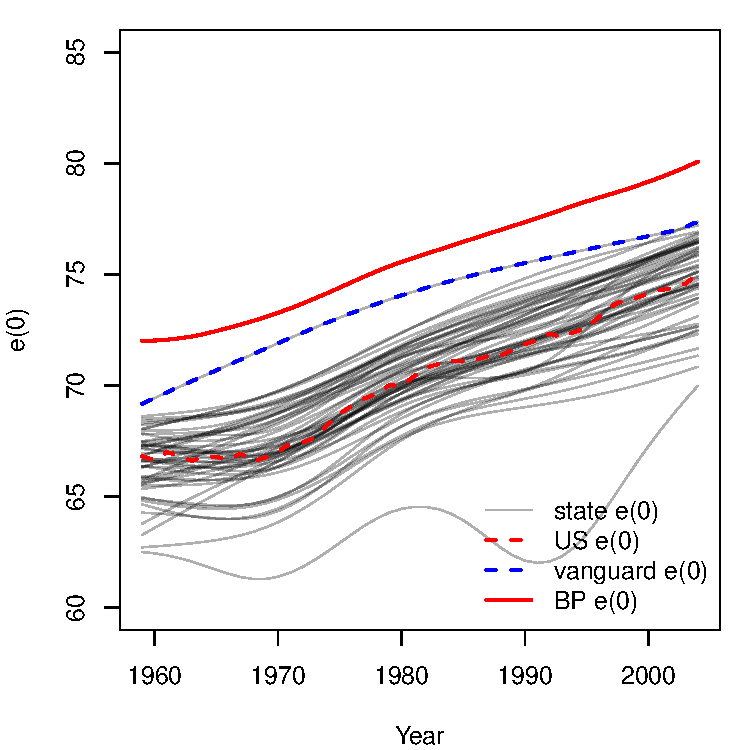
\includegraphics[scale=0.5]{Figures/e0trendsM.pdf}
\end{subfigure}
~
\begin{subfigure}[b]{.48\textwidth}
\centering
\caption{Females}
\label{fig:e0f}
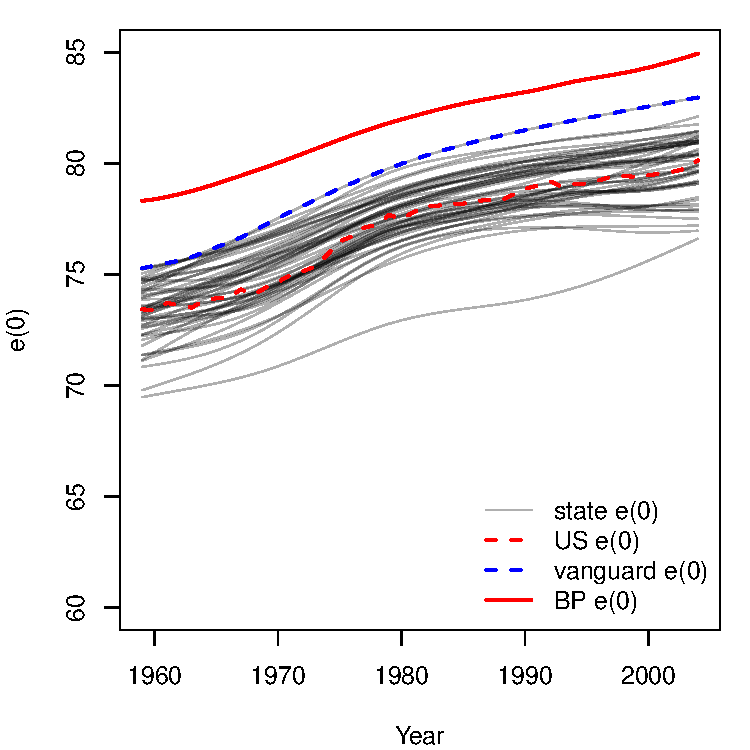
\includegraphics[scale=0.5]{Figures/e0trendsF.pdf}
\end{subfigure}
\end{figure}

If we take the mean rate of improvement for national or best practice trends,
and compare it with the means of each series, we can roughly conclude that the
best practices trend in year $t$ is a decent estimate of the national life
expectancy in 30 or so years. This time lag is valid for the present series,
but will vary depending on the number of cause groups that enter into the
selection of minimum mortality rates. Clearly, if the population units were
counties rather than states, the level of best practices life expectancy would
increase even further, but we opine that cause-specific smoothing at the county
level is more of a modelling gesture than sound practice, due to very low counts of deaths in
most counties in the U.S. In the final paper we will aim to test the cause set
proposed by \citet{vallin2008minimum} and compare it with other reasonable
configurations for the U.S., and so recommend a rule of thumb grouping.

\FloatBarrier
\subsection*{State differences by cause}

We decompose the state departures in life expectancy from the best practice
trend in each year and sex, over both age and cause. Part of the attraction of decomposing with respect to the best practices life expectancy is that contributions are always
of the same sign, which makes interpretation of the heatmap more intuitive.
Deeper shades of red indicate larger departures. In Figure~\ref{fig:dep}
we aggregate over age and average within decades to summarize the total
contribution to the departure from best practices.\footnote{The 2000s trend is
based on the average for the years 2000-2004 only.} Major causes of death are in
rows, and decades are organized in columns.

For the case of cardiovascular disease
and other causes, grouping departures into the 2$+$ group blends out much
interstate variation, since some contributions range as high as 4
years, but broad patterns are still visible.\footnote{This visual display may be
significantly adapted when we add more causes to the decomposition. We will also do a similar small multiples
display for grouped age patterns.}

Since the cause groupings available at the time of submission are not the final groupings, and
because the causes included in the study contribute such varying magnitudes to
state differences, trends are dominated by Cardivascular diseases and the large
aggregate group of all other causes. The 11 original causes were grouped into
five so as to make state patterns more visible. More commentary to come at a
later date.

\begin{figure}[t!]
\caption{State departures from vanguard $e(0)$ by large cause groups,
1959-2004.}
\label{fig:dep}
\centering
\begin{subfigure}[b]{\textwidth}
\centering
\caption{Males}
\label{fig:depm}
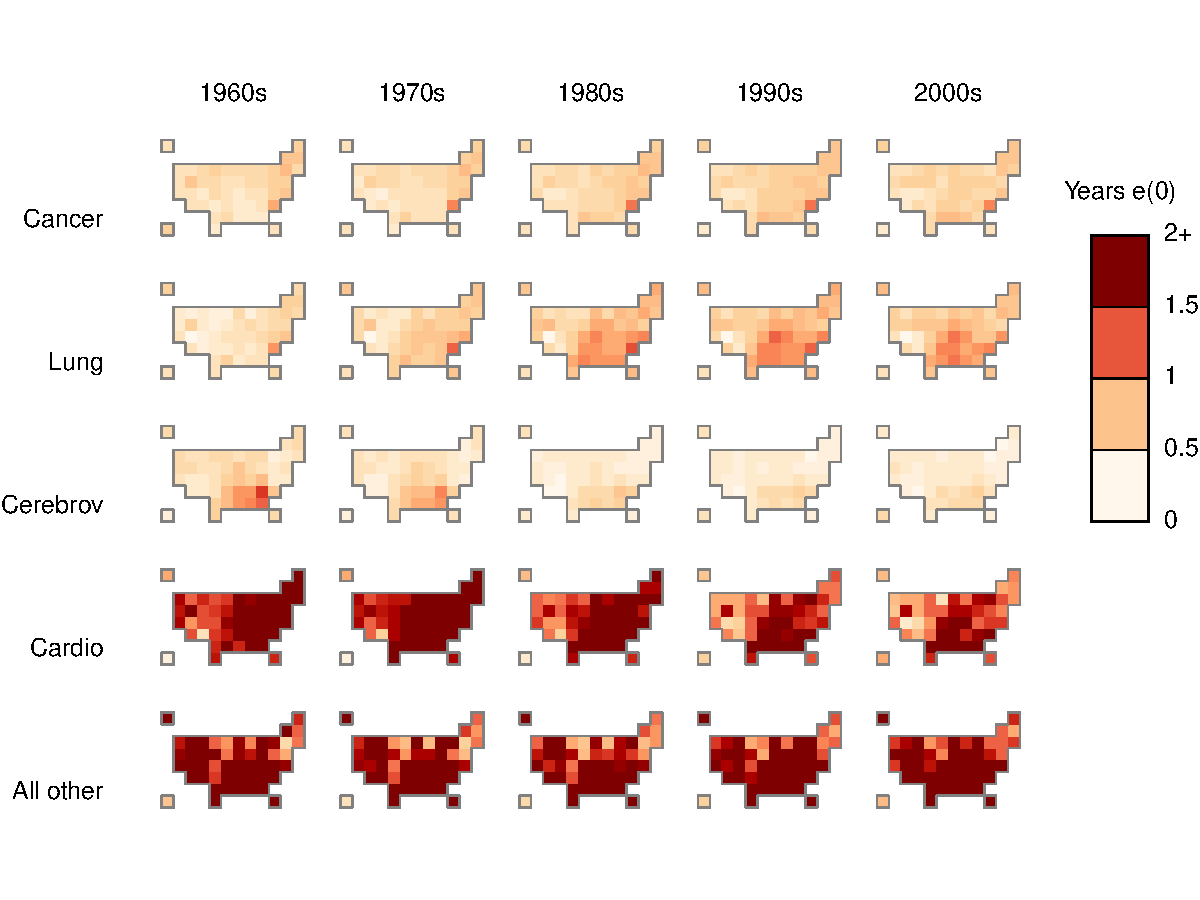
\includegraphics[scale=0.5]{Figures/StatesDecadesM.pdf}
\end{subfigure}
\\
\begin{subfigure}[b]{\textwidth}
\centering
\caption{Females}
\label{fig:depf}
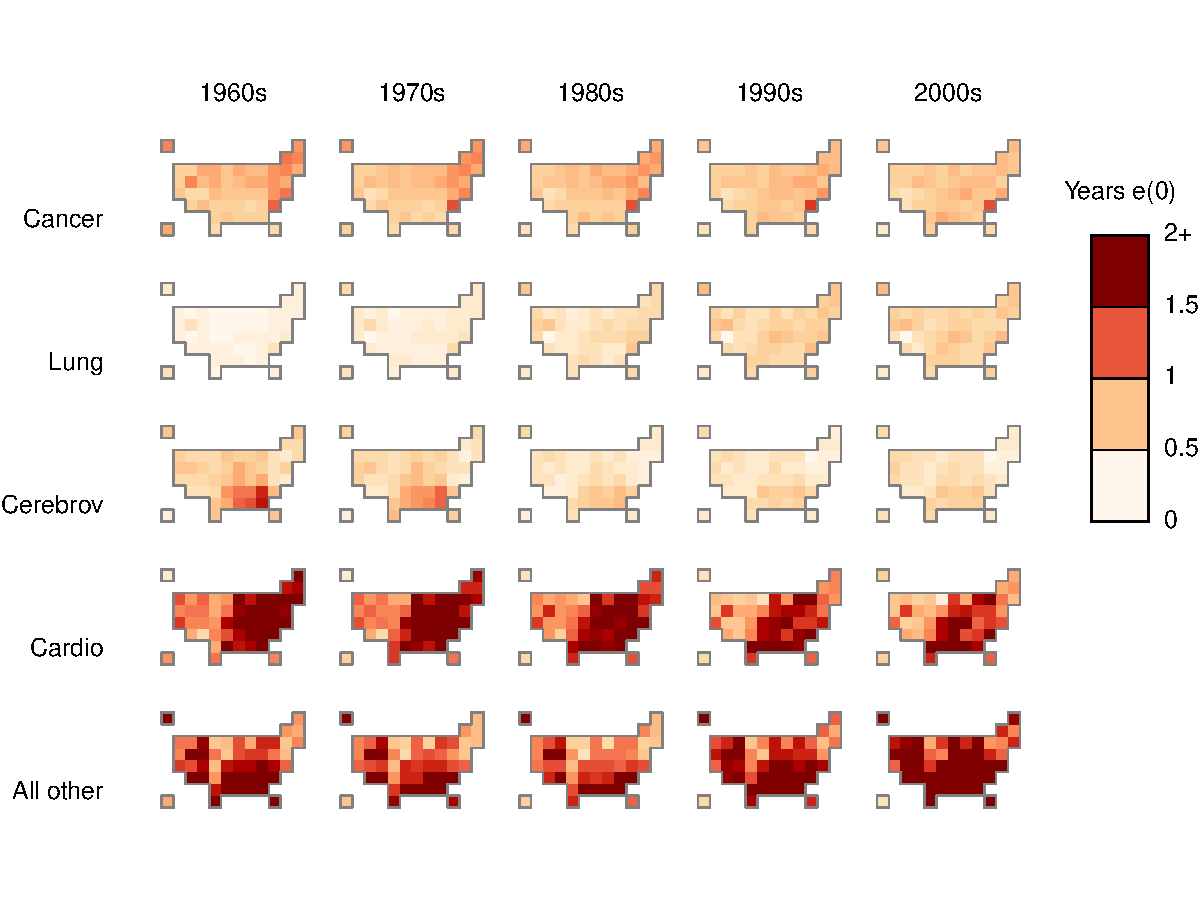
\includegraphics[scale=0.5]{Figures/StatesDecadesF.pdf}
\end{subfigure}
\end{figure}

\section*{}


\FloatBarrier

\bibliographystyle{plainnat}
%\bibliographystyle{demography}
  \bibliography{references.bib}   % Use the BibTeX file ``references.bib''.
\end{document}

